% anstelle von article auch KOMA-Skript-Variante scrartcl
\documentclass[11pt,twoside]{report}
%%anstelle von german auch ngerman
\usepackage{amsfonts,latexsym,eurofont,ngerman}
\usepackage{graphicx,color}

\usepackage[T1]{fontenc}
\usepackage[utf8]{inputenc}
\usepackage[ngerman]{babel}

%titelblatt
\thispagestyle{empty}

\setlength{\textheight} {270mm} 
\setlength{\textwidth} {150mm}

%Kopfzeile
\setlength{\topmargin} {-25mm}

%Fußzeile
%\setlength{\footheight} {10mm}
\setlength{\footskip} {10mm}


%Seiten link
\setlength{\oddsidemargin} {10mm} 

%Seite rechts und Rand
\setlength{\marginparwidth} {0mm} 
\setlength{\marginparsep} {0mm} 

%Absätze nicht einrücken, möglicherweise nicht zu empfehlen, falls viele Abbildungen vorhanden;
%Betreuer fragen
\parindent10mm

%Inhaltsverzeichnis
\usepackage[numindex,nottoc,section]{tocbibind} %Einbinden von Index-
                                %und Literaturverzeichnis (nummeriert) in das
                                %Inhaltsverzeichnis. Inhaltsverzeichnis wird 
                                %nicht eingebunden.


%anstelle von german auch ngerman
\usepackage{amsfonts,latexsym,eurofont,ngerman}
\usepackage{graphicx,color}

\usepackage[T1]{fontenc}
\usepackage[utf8]{inputenc}
\usepackage[ngerman]{babel}
\usepackage{fancyhdr} 

%titelblatt
\thispagestyle{empty}

\setlength{\textheight} {250mm} 
%\setlength{\textwidth} {140mm}

%Kopfzeile
\setlength{\topmargin} {-25mm}

%Fußzeile
%\setlength{\footheight} {10mm}
\setlength{\footskip} {10mm}


%Seiten links
%\setlength{\oddsidemargin} {10mm} 

% Randnotizen breite und Abstand zum Text
%\setlength{\marginparwidth} {0mm} 
%\setlength{\marginparsep}   {3mm} 

%Absätze nicht einrücken, möglicherweise nicht zu empfehlen, falls viele Abbildungen vorhanden;
%Betreuer fragen
%\parindent10mm

% Kopf- und Fußzeilen anpassen
\fancyhf{}  % Kopf- und Fußzeile leeren 
\fancyfoot[EL]{\thepage} 
\fancyfoot[OR]{\thepage} 
\renewcommand{\headrulewidth}{0pt}


%Inhaltsverzeichnis
\usepackage[numindex,nottoc,section]{tocbibind} 
%Einbinden von Index-und Literaturverzeichnis (nummeriert) in das Inhaltsverzeichnis. Inhaltsverzeichnis wird nicht eingebunden.

\usepackage{eso-pic,graphicx}
\usepackage{hyperref}
\hypersetup{pageanchor,linkcolor=black, colorlinks=true}

\makeatletter

\newcommand\BackgroundPicture[3]{%
  \setlength{\unitlength}{1pt}%
  \put(0,\strip@pt\paperheight){%
    \parbox[t][\paperheight]{\paperwidth}{%
      \vfill
      \centering\includegraphics[width=21.4cm,angle=45]
      {_Res/draft}
      \vfill
    }
  }
} 

\makeatother
\AddToShipoutPicture{\BackgroundPicture}


%\input{./Praxisprojekt_Dokument.tex}


\begin{document}


\begin{titlepage}
\author{}
%Bilder einfügen
\begin{figure}[hp]
	\centering
	\includegraphics[height = 13mm]{./_Res/RAC_Logo.jpg}
\end{figure}
\begin{center}
\huge
\textsc{Übersetzen von Schrittmotorprotokollen\\ mittels Mikrocontroller}\\

\vspace{2cm}

\LARGE
%\textsc{\bf Bachelorarbeit\\[0.5\baselineskip]
\textsc{\bf Praxisprojektbericht\\[0.5\baselineskip]
\Large \normalfont {im Studiengang Mess- und Sensortechnik\\[0.5\baselineskip]
Fachhochschule Koblenz, RheinAhrCampus Remagen}}

\large
\vspace{2cm}
\textnormal{vorgelegt von\\[0.5\baselineskip]\textbf{Johannes Dielmann}\\[0.5\baselineskip] geb.\ am 10.01.1984 in {\em Kirchen} }\\ 
\vspace{1cm}


\end{center}

\normalsize
\begin{flushleft}	

\vspace{15mm}
\begin{tabbing}
Externer Betreuer:\quad\=\kill
Betreuer: \> Prof.\ Dr.\ Carstens-Behrens\\[1\baselineskip]

\end{tabbing}
\end{flushleft}

%\vspace{0mm} 

\vspace{4cm}

\begin{center}
\textnormal{Remagen, \today}
\end{center}


\end{titlepage}

\pagestyle{fancy} 
% Erstellung des Inhaltsverzeichnisses
\thispagestyle{fancy}
\tableofcontents 	\newpage
\listoffigures 		\newpage
\listoftables		\newpage
\newpage

\section{Einleitung}
\subsection{Überblick}
Gegeben war das 3D-Lasererfassungssystem VI-900 der Firma Minolta, im Folgenden kurz VI-900 genannt, und ein Drehtisch. Der Drehtisch dient zur Aufnahme des zu erfassenden Objektes aus allen Richtungen. Des weiteren lässt sich das 3D-Modell später in der Software wesentlich einfacher zusammenführen wenn der Drehtisch benutzt wird.\\
Dem VI-900 lag die Software RapidForm2004 bei. Mit dieser Software lassen sich 3D-Modelle einfach bearbeiten und einzelne Modelle zu einem gesamten zusammenführen. Diese Software spricht sowohl das VI-900 an als auch den Drehtisch. \\
In RapidForm2004 sind jedoch nur einige wenige Schrittmotoren und deren Protokolle hinterlegt.
\subsection{Aufgabenstellung}
Mit dem Aufbau aus RapidForm2004, Lasererfassungssystem und Drehtisch sollen auf einfachem Wege 3D-Modelle eines Objektes erzeugt werden und diese dann zur Vermessung oder zur weiteren Verwendung in CAD-Software herangezogen werden.\\
Um ein vollständiges und brauchbares 3D-Objekt zu erhalten kann die Software einen Drehtisch ansteuern.\\
Da das Protokoll des Drehtisches nicht kompatibel zu denen in der Software war musste das Protokoll also übersetzt werden.
\subsection{Problemlösung}
Da die Kommunikation mittels ASCII-Zeichen über die RS-232 Schnittstelle des Computers erfolgt, lässt sich die Information leicht mit einem Mikrocontroller abfangen, auswerten und richtig kodiert an die Ansteuerung des Drehtisches weitersenden.
Benötigt wird also ein Mikrocontroller mit 2 RS-232 Schnittstellen. Um später den Ablauf anzeigen zu können und den Drehtisch auch manuell bedienen zu können wurde noch ein LC-Display und mehrere Bedientaster eingeplant.\\
Da die Ansteuerung des Schrittmotors als Einschub für ein 19"-Rack realisiert ist wählte ich für den Mikrocontroller auch die Realisierung als 19"-Einschubplatine.  \marginpar{Eine Randnotiz}
\newpage

\section{Projektaufbau}
\subsection{Übersicht}
\begin{figure}[hp]
	\centering
	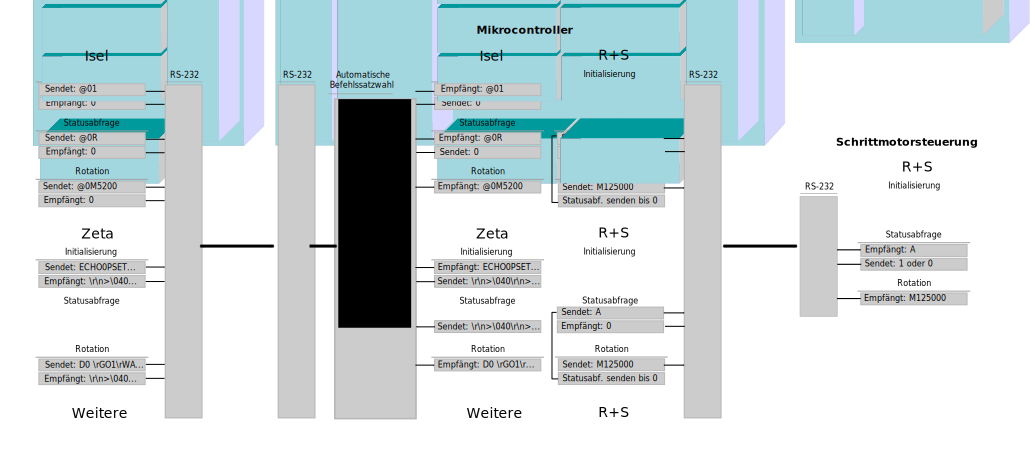
\includegraphics[width=10cm]{./_Res/Uebersicht.jpg}
	\caption{Übersicht}
\end{figure}
\subsection{Die einzelnen Komponenten}
//TODO Fußnoten für Komponenten, Hersteller und Websites\\
//TODO Komponenten auf Abbildung erwähnen!
\subsubsection{Lasererfassungssystem VI-900}
Das Lasererfassungsystem VI-900 der Firma Minolta besteht aus einem Lasertriangulator und einer Kamera. Das System lässt sich über eine SCSI Schnittstelle ansprechen und konfigurieren. Zur mobilen Nutzung kann das Gerät  \marginpar{Eine Randnotiz} auch auf der Rückseite eingestellt werden. Aufgenommene Daten können auf einer CF-Karte gespeichert werden. Im Projekt wurde jedoch lediglich die Ansteurung via SCSI genutzt.
\subsubsection{Drehtisch}
Der Drehtisch ist eine Eigenkonstruktion der Werkstatt des RheinAhrCampus. Er besteht aus einer massiven Edelstahl Arbeitsplatte, welche auf 4 Füßen ruht. Aus dieser ist eine //TODO Welche form?? ausgeschnitten. In diesem Ausschnitt befindet sich, auf einem Zweischienensystem gelagert, der Drehtisch. Mit dem Schienensystem lässt der Drehtisch sich in der Vertikalen positionieren. Mit einem Schrittmotor lässt sich der Drehtisch in der Höhe verstellen. Ein weiterer Schrittmotor ist für die Drehung des Tisches zuständig. //TODO Getriebe erklären!  
\subsubsection{Ansteuerung für Drehtisch}
Die Ansteurung für den Drehtisch besteht aus einem 19"-Rack. In diesem ist ein ATX-PC-Netzteil verbaut. Außerdem sind 2 Einschubkarten der Firma R+S vorhanden. Die Karten sind sogenannte Stepper-Karten. Diese übernehmen komfortabel die Ansteuerung der beiden Schrittmotoren. Mittels RS-232 Schnittstelle lassen sich die Karten konfigurieren und ansteuern. Die Konfiguration und Ansteuerung erfolgt über einen vorgegeben ASCII Befehlssatz. Außerdem können 2 oder mehr Karten als "Daisy-Chain" zusammengeschaltet werden. 
//TODO Daisy-Chain erklären und Konfiguration genauer beschreiben.
\subsubsection{Entwicklerboard STK500}
Um den eingesetzten Mikrocontroller zu programmieren und die Programmierung zu überprüfen wurde mir das Entwicklerboard STK500 der Firma ATMEL zur Verfügung gestellt. Das Board enthält mehrere Mikrocontroller Steckplätze, 2 Serielle Schnittstellen, 8 Taster, 8 LEDs, 2 Erweiterungsports, ein integriertes Programmiersystem //TODO besserer Name! und mehrere Jumper zum konfigurieren des Boards.\\
Von den beiden seriellen Schnittstellen kann die eine zur Programmierung des Mikrocontroller verwendet werden. Die andere kann zur Kommunikation mit dem Mikrocontroller genutzt werden.\\
Auf dem Board stehen 5 10 polige Pinheader\footnote{Eine Stiftleiste (engl. pin header) ist ein Steckverbinder mit mehreren in Reihe angeordneten Stiftkontakten, der auf Leiterplatten in der Elektronik Verwendung findet. Sie hat den Zweck, eine Verbindung mit vielen Kontakten von einer Platine zu einer anderen oder zu peripheren Baugruppen herzustellen, meist mit Hilfe von Flachbandkabeln und Pfostenverbindern oder einer Buchsenleiste. }  //TODO Fußnote für Pinheader 
Die Taster und de LEDs können jeweils mit einem 10 poligen Flachbandkabel mit dem zugehörigen Pinheader des Mikrocontroller verbunden werden. // TODO evtl Grafik einfügen 
\subsubsection{Mikrocontroller}

\subsubsection{Entwicklungs PC}

\subsubsection{Erfassungs PC}
\newpage

\addcontentsline{toc}{section}{A Anhang 1}
\section*{A Anhang 1}
\newpage

\begin{thebibliography}{99}
%Zeitschriftenartikel
\bibitem{maquarbra} Mack, T., Quarg, G., Braun, C.\ (2006). {\em The mean square error of prediction in the chain ladder reserving method. A comment.} ASTIN Bulletin 36, 543-553. 
%Buch
\bibitem{mik} Mikosch, T.\ (1994). {\em Non-life insurance mathematics.} Springer, Heidelberg.
\end{thebibliography}
\newpage

\section*{Erklärung}

\vspace{2cm}

Hiermit versichere ich, dass ich den vorliegenden Bericht selbständig und nur unter Verwendung der angegebenen Quellen und Hilfsmittel verfasst habe.

\vspace{2cm}

Remagen, den \today \hfill {Johannes Dielmann} 
\begin{figure}[hp]
	\hfill
	\includegraphics[height = 13mm]{../../../../Unterschrift.png}
\end{figure}


\end{document}
